\chapter{Local Feature Matchers}










\section{Experimental Setup and Results}

The experiments evaluated BFMatcher and FLANN for time efficiency, accuracy, and robustness across diverse, real-world datasets. Other stages of the pipeline, were optimized to ensure fair comparisons between the matchers.
Metrics included Mean Absolute Error (MAE) of the GPS estimation and runtime in seconds. Mean heading error was excluded, as it was inferred through GPS error, and ground truth heading data was unavailable. 
Three testing stages were conducted: optimization to identify the best parameters, robustness to assess generalizability, and performance evaluation to compare the matchers under similar optimized conditions.


\subsection*{Optimization Testing}
The goal of optimization testing was to identify parameters that maximize performance without compromising generalizability. FLANN and BFMatcher were tested with different configurations, specifically Lowe’s ratio and cross-checking. 

Confidence thresholding, as noted earlier, was not pursued due to its sensitivity to parameter changes. RANSAC was tested separately within the pose estimation stages.

\subsubsection*{Test 1: Cross-Checking}

Both matchers were tested with cross-checking to improve accuracy by reducing false positives. Cross-checking ensures that matches are \textbf{mutual} in both directions between two images. However, due to \textbf{noise} and imperfections in real-world data, matching between images is inherently \textbf{asymmetrical}, meaning the top matches in one direction often differ significantly from those in the reverse direction.

Empirical testing showed that only \textbf{FLANN} had potential for practical use with cross-checking, as BFMatcher’s built-in cross-checking was too slow for real-time application. Despite attempts to optimize FLANN with cross-checking, the combined impact of noise, asymmetry, and computational costs limited its effectiveness. The results are summarized below.

\textbf{Initial Approach}
Initially, cross-checking was applied \textbf{after Lowe’s ratio filtering}. However, this resulted in poor accuracy across \textbf{4 out of 5 datasets}. Applying Lowe’s ratio first left too few matches for cross-checking, as the asymmetry between matching directions caused many mutual matches to be lost. As a result, the approach became unstable and unreliable. Table~\ref{tab:flann_comparison} summarizes the comparison.

\begin{table}[H]
    \centering
    \begin{tabular}{|c|c|c|c|c|c|c|}
    \hline
    \makecell{\textbf{Matcher}} & 
    \makecell{\textbf{Metric} \\ \textbf{Type}} & 
    \makecell{\textbf{CITY1}} & 
    \makecell{\textbf{CITY2}} & 
    \makecell{\textbf{ROCKY}} & 
    \makecell{\textbf{DESERT}} & 
    \makecell{\textbf{AMAZON}} \\
    \hline
    \multirow{2}{*}{\makecell{FLANN \\ (No Cross-Check)}} & 
    \makecell{MAE GPS \\ (m)} & 56.59 & 4.70 & 14.63 & 71.20 & 32.35 \\
    \cline{2-7}
    & \makecell{Runtime \\ (s)} & 42.72 & 41.61 & 41.96 & 43.42 & 53.62 \\
    \hline
    \multirow{2}{*}{\makecell{FLANN \\ (With Cross-Check)}} & 
    \makecell{MAE GPS \\ (m)} & 70.71 & 7.96 & 23.64 & 41.37 & 44.39 \\
    \cline{2-7}
    & \makecell{Runtime \\ (s)} & 71.60 & 72.28 & 88.99 & 70.98 & 62.28 \\
    \hline
    \end{tabular}
    \caption{Comparison of FLANN with and without Post-Lowe’s Cross-Check across Datasets (MAE GPS and Runtime)}
    \label{tab:flann_comparison}
\end{table}


\textbf{Experimenting with Pre- and Post-Lowe’s Filtering}
However, in the desert dataset, there were significant improvements. To explore this further, three strategies were explored to attempt to help the cross-checking process generalize better across datasets. These strategies tested variations of a relaxed Lowe's threshold prior to cross-checking, to reduce computational load without removing too many matches. After cross-checking, a set stricter Lowe's threshold was applied to remove false positives.

\begin{itemize}
    \item \textbf{Low or No Pre-Filtering:}  
    Minimal filtering allowed sufficient matches to pass to cross-checking, but resulted in unacceptable runtimes.

    \item \textbf{High Pre-Filtering:}  
    Aggressively filtering matches reduced runtime but led to instability and poor results across most datasets, as too few matches remained. There were no static parameters that could balance this trade-off.

    \item \textbf{Dynamic Pre-Filtering:}  
    Lowe’s ratio was incremented dynamically until \textbf{n matches} were found. \textit{n} was tuned to achieve maximum acceptable runtime. Although this method ensured stability, it did not improve accuracy over no cross-checking in \textbf{4 out of 5 datasets}.
\end{itemize}

\subsubsection{Testing Conclusion}
Cross-checking was tested thoroughly but failed to consistently improve performance with any combination of pre- and post-filtering. Its effectiveness was limited by asymmetry in the matching process and the characteristics of the datasets used. As a result, a generalizable increase in accuracy could not be achieved in real-time. Therefore, cross-checking was not adopted. 




\subsubsection{Test 2: Lowe’s Ratio Test}  

Lowe’s ratio was employed to reduce ambiguity by comparing the best and second-best matches for each keypoint. A match was retained if the ratio between these distances fell below a defined threshold. This method effectively filtered false positives, ensuring only distinct matches were kept. However, determining an optimal static threshold was challenging, as performance varied across different datasets and feature extraction methods.

During testing, the optimal static threshold was found to be 0.8 for AKAZE and 0.7 for ORB, with slight variations depending on other parameters. These values improved accuracy but lacked generalizability across datasets that differed in keypoint density and quality. Consequently, a dynamic approach was implemented, adjusting the threshold iteratively until a minimum number of matches were obtained to ensure stability. The initial thresholds and increment steps were tuned to have minimal influence in most cases, aiming to preserve the generalizability of the method. This dynamic method better balanced quality and efficiency than fixed thresholds.

While dynamic tuning enhanced performance, it compromised generalaizbility. Future iterations could benefit from real-time threshold adjustments to adapt to changing conditions in-flight or during GPS loss, maintaining both generalizability and accuracy.





\subsection{Robustness Evaluation}

The robustness tests assess the matchers' ability to generalize, in terms of accuracy and performance, across diverse datasets and non-ideal conditions, ensuring reliability in real-world applications. These tests explore the impact of noisy keypoints through various detector thresholds and limited post-match filtering, providing insights into the matchers' ability to ensure accurate matches under challenging conditions.

\subsubsection*{Test 1: Robustness Evaluation Under Limited Post-Filtering}

This robustness test evaluates the performance of BFMatcher and FLANN without using Lowe’s ratio or other ambiguity-filtering techniques. However, RANSAC and other downstream processes were applied to maintain accuracy in the estimation stages. The same keypoints were passed into the matching stage to ensure a fair comparison. The primary goal was to observe the raw quality and number of matches produced by each matcher. The results are summarized in Table~\ref{tab:robustness_lowes_comparison}.

\begin{table}[H]
    \centering
    \begin{tabular}{|c|c|c|c|c|c|c|}
    \hline
    \makecell{\textbf{Matcher}} & 
    \makecell{\textbf{Metric} \\ \textbf{Type}} & 
    \makecell{\textbf{CITY1}} & 
    \makecell{\textbf{CITY2}} & 
    \makecell{\textbf{ROCKY}} & 
    \makecell{\textbf{DESERT}} & 
    \makecell{\textbf{AMAZON}} \\

    \hline
    \multirow{4}{*}{\makecell{BFMatcher}} & 
    \makecell{MAE \\ GPS (m)} & 777.64 & 507.75 & 465.81 & 534.85 & 319.65 \\
    \cline{2-7}
    & \makecell{Runtime \\ (s)} & 140.56 & 145.91 & 115.26 & 108.71 & 192.19 \\
    \cline{2-7}
    & \makecell{Mean \\ Matches} & 9036.15 & 9062.00 & 10416.30 & 6460.95 & 10451.65 \\
    \cline{2-7}
    & \makecell{Mean \\ Keypoints} & 9059.20 & 9041.27 & 10429.07 & 6480.47 & 10479.13 \\
    \hline

    \multirow{4}{*}{\makecell{FLANN}} & 
    \makecell{MAE \\ GPS (m)} & 826.73 & 526.42 & 471.96 & 539.96 & 340.21 \\
    \cline{2-7}
    & \makecell{Runtime \\ (s)} & 50.88 & 46.10 & 50.39 & 50.69 & 64.91 \\
    \cline{2-7}
    & \makecell{Mean \\ Matches} & 9045.45 & 9063.75 & 10434.75 & 6507.80 & 10479.50 \\
    \cline{2-7}
    & \makecell{Mean \\ Keypoints} & 9059.20 & 9041.27 & 10429.07 & 6480.47 & 10479.13 \\
    \hline
    \end{tabular}
    \caption{Performance Comparison of BFMatcher and FLANN Under Limited Post-Filtering}
    \label{tab:robustness_lowes_comparison}
\end{table}

\textbf{Observations}
\begin{itemize}
    \item \textbf{Performance Comparison:}  
    BFMatcher achieved slightly better accuracy across most datasets. However, the improvements were marginal compared to the significant variation in runtime, with BFMatcher taking two to three times longer than FLANN across all datasets.

    \item \textbf{Matches Found:}  
    Both matchers detected a similar number of matches, indicating that the primary difference lies in match quality. BFMatcher’s exhaustive approach yields higher-quality matches but at the cost of substantial runtime.

    \item \textbf{Implications:}  
    In most cases, the minor accuracy improvements offered by BFMatcher do not justify its high computational cost. FLANN remains the better option for real-world applications, where runtime efficiency is critical.
\end{itemize}




\subsubsection*{Test 2: Robustness Evaluation Under Different Detector Thresholds}

This test evaluates the performance of BFMatcher and FLANN under varying keypoint thresholds to assess the differences in accuracy, stability, and scalability. The goal is to determine how the two matchers perform across a range of detection thresholds—from low to high keypoints—and to observe whether the methods converge or diverge at specific higher levels. This test is also essential to identify the stability of the methods at low keypoints. The results are summarized in Figure~\ref{fig:divergence_plot}.

\begin{figure}[H]
    \centering
    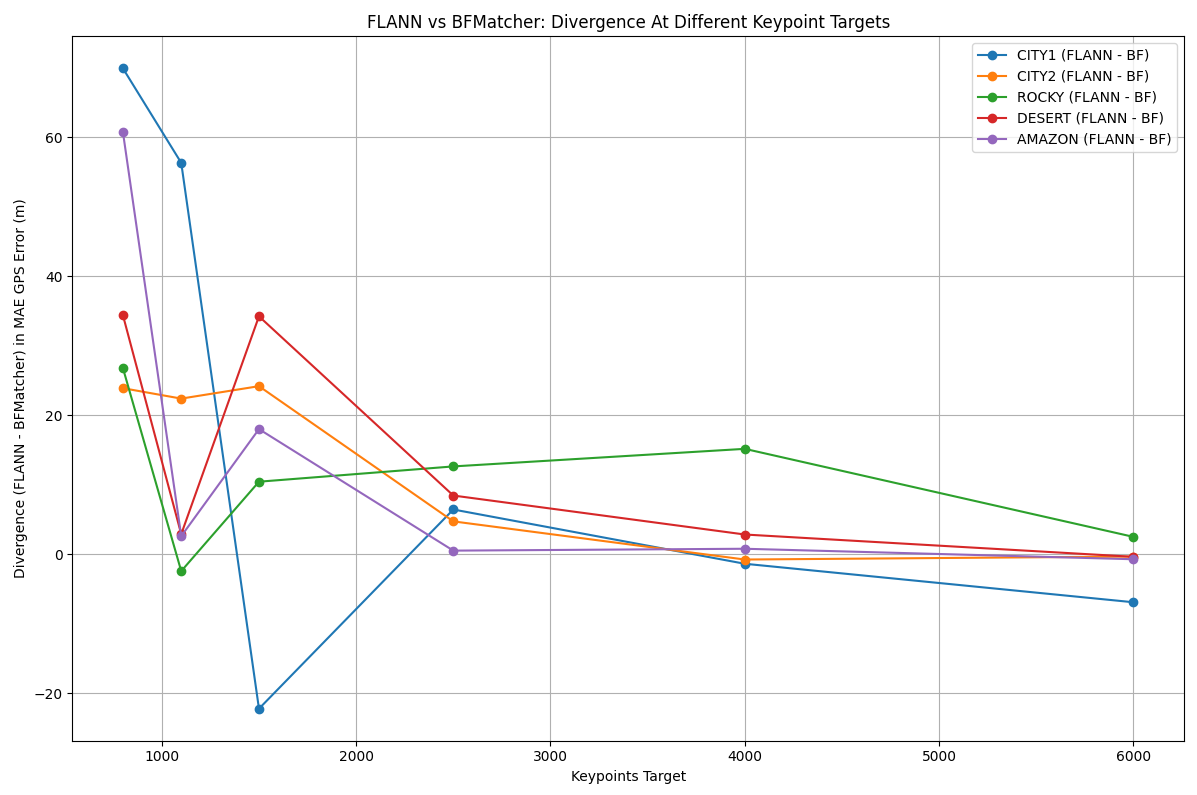
\includegraphics[width=\textwidth]{./Graphs/Divergence_BF_FLANN_KPS.png}
    \caption{Divergence in MAE GPS Error Between FLANN and BFMatcher Across Keypoint Targets.}
    \label{fig:divergence_plot}
\end{figure}

\textbf{Observations}

\begin{itemize}
    \item \textbf{Divergence and Convergence:}  
    As the number of keypoints increases, the difference in MAE GPS error between BFMatcher and FLANN decreases, showing that both matchers converge to similar levels of accuracy. At higher keypoint counts, the performance gap becomes negligible, with both methods providing comparable accuracy. Beyond 5000 keypoints, the error difference is minimal, well within acceptable limits for real-time applications.

    \item \textbf{Match Quantity vs Quality:}  
    Both matchers identified a similar number of matches in most tests, but the main distinction was in match quality. BFMatcher's exhaustive approach produced slightly higher-quality matches but required more processing time. FLANN, however, provided competitive accuracy with significantly faster runtimes, maintaining acceptable match quality.

    \item \textbf{Lowe's Ratio and Abnormalities:}  
    FLANN outperformed BFMatcher in several cases, primarily due to the effects of Lowe's filtering. Specifically:
    \begin{itemize}
        \item When Lowe's ratio was too lenient, incorrect matches could pass, but FLANN's approach often filtered these out by not identifying a suitable second match.
        \item When Lowe's ratio was too strict, valid matches could be discarded if the second-best match was too similar, but FLANN occasionally allowed these through by selecting slightly lower-quality second matches.
    \end{itemize}
    This demonstrates the limitations of static thresholds in Lowe's ratio and highlights the potential issues with overly rigid filtering.

    \item \textbf{Accuracy and Scalability:}  
    Both matchers showed decreasing error rates as the number of keypoints increased, improving overall stability. However, BFMatcher’s runtime increased much faster than FLANN's as the keypoint count grew, making FLANN a better option for handling larger datasets efficiently.

    \item \textbf{Implications:}  
    As keypoint counts rise, both matchers achieve comparable accuracy, but FLANN's superior efficiency and scalability make it the more practical choice for large-scale, real-time applications, balancing accuracy with computational cost.
\end{itemize}



\subsection*{4.3 Accuracy and Runtime Evaluation}

This evaluation compares the accuracy and runtime of BFMatcher and FLANN using optimized parameters for each dataset and matching method. The goal is to assess their trade-offs between precision and computational efficiency. Results are summarized in Table~\ref{tab:flann_bf_comparison}.

\begin{table}[H]
    \centering
    \begin{tabular}{|c|c|c|c|c|c|c|}
    \hline
    \makecell{\textbf{Matcher}} & 
    \makecell{\textbf{Metric Type}} & 
    \makecell{\textbf{CITY1}} & 
    \makecell{\textbf{CITY2}} & 
    \makecell{\textbf{ROCKY}} & 
    \makecell{\textbf{DESERT}} & 
    \makecell{\textbf{AMAZON}} \\
    \hline
    
    \multirow{2}{*}{\makecell{FLANN}} & 
    \makecell{MAE GPS \\ (m)} & 56.59 & 4.70 & 14.63 & 71.20 & 32.35 \\
    \cline{2-7}
    & \makecell{Runtime \\ (s)} & 42.72 & 41.61 & 41.96 & 43.42 & 53.62 \\
    \hline

    \multirow{2}{*}{\makecell{BF}} & 
    \makecell{MAE GPS \\ (m)} & 53.89 & 3.79 & 16.36 & 68.64 & 33.24 \\
    \cline{2-7}
    & \makecell{Runtime \\ (s)} & 203.49 & 228.59 & 46.33 & 52.59 & 88.95 \\
    \hline
    
    \end{tabular}
    \caption{Performance comparison of optimized BFMatcher and FLANN Across Datasets}
    \label{tab:flann_bf_comparison}
\end{table}

\textbf{Observations}
\begin{itemize}
    \item \textbf{BFMatcher} achieved slightly better MAE in some cases, but this precision came at the cost of significantly longer runtimes, with execution times often more than double those of FLANN.
    
    \item \textbf{FLANN} maintained faster runtimes across all datasets, demonstrating better computational efficiency, though with marginally higher MAE values in some scenarios.


    \item \textbf{Test conclusion:} FLANN is more suited for real-time applications, offering a practical balance between speed and accuracy, with scalability to handle larger datasets efficiently.
\end{itemize}




\section*{Conclusion} 
This study evaluated BFMatcher and FLANN for local feature matching. BFMatcher provided slightly higher-quality matches but was computationally expensive and more stable when fewer keypoints were available. FLANN, however, delivered comparable accuracy with significantly better runtime and scalability, making it ideal for real-time applications when sufficient keypoints are available.

In practice, with modern computational power generating high keypoint counts, the differences between the two methods become negligible. While BFMatcher shows more robustness under low-keypoint conditions, its lack of scalability makes it less practical compared to FLANN, which provides a more efficient solution without compromising accuracy.


\section*{Future Work} 
Future research should focus on: 
\begin{itemize} 
    \item \textbf{Adaptive Filtering:} Develop dynamic filtering techniques and inference models for determining optimal Lowe's threshold to address its limitations.  
    \item \textbf{Extreme Testing:} Explore the matchers' performance under more severe environmental conditions to improve robustness.  
    \item \textbf{Neural Network Integration:} Investigate ways to efficiently integrate learning-based matchers like LightGlue into real-time systems.
\end{itemize}

These improvements will enhance the robustness, efficiency, and applicability of feature matching in future systems.


\newpage